\documentclass[12pt, english]{article}

% Language setting
% Replace `english' with e.g. `spanish' to change the document language
\usepackage[english]{babel}

% Set page size and margins
% Replace `letterpaper' with`a4paper' for UK/EU standard size
\usepackage[letterpaper,top=2cm,bottom=2cm,left=3cm,right=3cm,marginparwidth=1.75cm]{geometry}

% Useful packages
\usepackage{amsmath}
\usepackage{graphicx}
\usepackage[colorlinks=true, allcolors=blue]{hyperref}

\title{Fantasy Predictor}
\author{Kyle Davis}

\begin{document}
\maketitle

\begin{abstract}
The examination of the offensive fantasy baseball predictor has unveiled a complex interplay of predictive capabilities, strengths, and challenges in player performance forecasting. This study delves into the model's efficacy, emphasizing the necessity for tailored strategies in player selection and draft success within the fantasy baseball domain. Key variables such as hard hit rate, contact rate, home run to fly ball ratio, and games played serve as robust predictors, highlighting the model's utility in forecasting player success and evaluating performance trajectories. While obstacles persist in accommodating players without major league statistics, ongoing refinement targeting age-related dynamics is essential for enhancing predictive accuracy. The convergence of public and proprietary analytics presents an opportunity for advancement in baseball predictive analytics, advocating for collaboration, innovation, and knowledge sharing to improve accuracy and strategic decision-making. By fostering a culture of continuous innovation and precision, researchers can propel predictive models to become indispensable tools for informed decision-making and competitive success in the dynamic realm of fantasy baseball analysis.
\end{abstract}
\vfill{}


\pagebreak{}

\section{Introduction}

In the realm of fantasy baseball, where strategic decisions hinge on predicting player performance with precision, the quest for an offensive fantasy baseball predictor has been a perennial challenge. This paper delves into the development and refinement of a tool aimed at predicting fantasy output in my league specifically which will here fourth be referred to as Hectorball.

The allure of fantasy baseball lies in its fusion of statistical analysis and sports fandom, offering participants the opportunity to construct virtual rosters based on real-world player performances. However, the key to success in this realm often rests on the ability to anticipate player outcomes with accuracy, particularly in the offensive domain where hits, home runs, and RBIs reign supreme.

Against this backdrop, the emergence of a novel offensive fantasy baseball predictor stands as a testament to the intersection of data science, sports analytics, and predictive modeling. By harnessing the power of advanced algorithms and historical performance data, this predictor aims to provide users with invaluable insights into player projections, enabling them to make informed roster decisions and gain a competitive edge in their fantasy leagues. There are dozens of predictors out there from ESPN, to Fantrax, and more advanced ones that are not specific to fantasy like ZiPS, Steamer, and so many more.

Through a detailed exploration of the development process, from conceptualization to implementation, this paper sheds light on the inner workings of the offensive fantasy baseball predictor, unraveling the intricacies of its design, methodology, and predictive capabilities. 
Each league possess their own rules, scoring and penalizing players for various things such as home runs, strike outs, RBI's and much more. Hectorball is extremely unique in that it does not reward RBI's and punish for strike outs. Hectorball was originally created in the 1980's and has been around every year since. It is a keeper league meaning that you keep a set amount of players every year and then draft to fill out the remaining spots. Hectorball is designed to create the most realistic scoring system in fantasy, not counting for typical fantasy stats like runs and RBI's since those can hinge on the players real team. Hectorball is a very competitive league with many of the original owners still a part of the league, and many newer ones such as myself. I have never made it past the first round of the playoffs so I needed a predictor that would help me get there.  This is why predictors have never been of much use to me and has led for me to use my own predictor.



\section{Literature Review}

In the study by Lyle (2007), the focus was on enhancing player performance predictions in baseball through a comprehensive exploration of machine learning techniques. By amalgamating statistical data from the past thirty years, the research aimed to refine projections for key offensive statistical categories. The results demonstrated that leveraging machine learning methodologies could yield prediction accuracies on par with some of the top-tier existing systems. The study not only constructed a robust baseball prediction system using diverse machine learning approaches but also delved into the comparative analysis of prediction systems, showcasing the efficacy of ensemble learning techniques like bagging, boosting, and stacking. Furthermore, the study emphasized the significance of tailoring machine learning techniques to specific statistical categories, highlighting the variability in predictive performance across different offensive metrics. Ultimately, the research underscored the importance of utilizing innovative approaches, such as training and testing prediction systems based on a limited dataset comprising the one hundred sixty-two games preceding the target season, which proved to be a viable strategy for achieving comparable prediction accuracy when compared to systems with more extensive data sources.

In the study conducted by Huddleston (2012), the primary objective was to investigate the relative value of pitchers versus hitters in a fantasy baseball league using hierarchical Bayesian models. The research compared three models, one of which distinguished between pitchers and hitters without further differentiation, another which differentiated between starting and relief pitchers, and a third model that made no distinction between hitters and pitchers. Utilizing Bayesian goodness-of-fit tests, the study revealed that the data exhibited a slight right-skewed distribution, suggesting the suitability of a probability distribution like the gamma distribution. The second model, which compared pitchers and hitters without distinguishing between pitcher types, emerged as the superior model based on the Deviance Information Criterion (DIC). Posterior predictive densities for specific players indicated that pitchers, including Kershaw, Lincecum, Lester, and Latos, consistently outperformed hitters in terms of weekly point totals. Despite the presence of top fantasy hitters like Ellsbury and Bautista in the roster, pitchers demonstrated higher weekly performance on average. This analysis provides valuable insights into player dynamics and strategic decision-making in fantasy baseball leagues, offering a foundation for further exploration utilizing advanced statistical modeling techniques within this domain.

Riley's study (2012) delves into the realm of forecasting sporting event outcomes, specifically focusing on predicting baseball game results through diverse machine learning algorithms encompassing classification and regression methodologies. The research highlights the potential of utilizing Major League Baseball's (MLB) gameday data, which offers comprehensive insights into every pitch thrown during games, including speed, trajectory, and break. By analyzing pitcher-hitter tendencies from this rich dataset, the study aimed to enhance performance predictions. A notable gap identified was the limited incorporation of fielding and defensive data, with fielding percentage deemed insufficient in evaluating defensive effectiveness, especially in cases where players have restricted range despite high fielding percentages. The study suggests the incorporation of external features beyond traditional baseball statistics, such as Twitter sentiment analysis, to potentially augment prediction accuracy. While the viability of deriving meaningful signals from Twitter data for regular season MLB games remains uncertain, this exploration opens avenues for leveraging diverse data sources to enhance outcome predictions in baseball.

Elfrink's study (2018) delves into predicting individual MLB game outcomes using historical data and various machine learning algorithms like random forests and XGBoost. The research aimed to determine if it's possible to forecast which team will emerge victorious in baseball games. Among the algorithms tested, XGBoost exhibited the highest accuracy at 0.5552, indicating room for improvement with more data, enhanced computational resources, and refined feature engineering techniques. Despite the inherent unpredictability of baseball games, the study revealed that predictive models outperformed random guessing, suggesting that pre-game information could serve as an indicator of game outcomes. Surprisingly, the regression approach did not yield superior results compared to the classification method. Additionally, adding numerous features related to recent statistics led to performance deterioration, possibly due to noise in the data overwhelming the algorithms. While the results didn't surpass those of betting companies, the study proposed potential enhancements in feature engineering and model refinement to achieve competitive outcomes. Overall, the research sheds light on the complexity of predicting MLB game results and underscores the significance of strategic data utilization in enhancing predictive capabilities within the realm of sports analytics.

Herlin's dissertation (2015) delves into the realm of predicting outcomes for fantasy baseball seasons, focusing on optimizing participant draft selections. The research utilizes a Bayesian approach alongside nonlinear growth curves and nonparametric regression tree methodologies to forecast player statistics and future outcomes. Building upon prior quantitative baseball research, the dissertation introduces a novel approach that blends parametric and non-parametric techniques to predict individual batting and pitching performances with a high degree of accuracy. The methodology incorporates unique factors like age effects, reversion, and team defense impact for pitchers, providing comprehensive forecasts that surpass traditional ranking systems. Notably, player-by-player simulations are integrated to project runs and RBI for batters, enhancing the accuracy of batting predictions significantly. While the pitching model competes with industry-leading projections, the batting model stands out as one of the most advanced in the field. Future extensions of this work could involve evaluating different lineup strategies, assessing potential trades in Major League Baseball, and incorporating additional metrics as fantasy baseball scoring evolves. This research contributes valuable insights into leveraging advanced statistical techniques to enhance fantasy baseball predictions and offers a robust framework for strategic decision-making in fantasy sports.

The study conducted by Weiss, Demski, and Backen (2011) delves into the controversy surrounding whether fantasy sports, specifically fantasy baseball, should be classified as a form of gambling. Utilizing the predominance rule, which defines an activity as gambling if outcomes rely more on chance than skill, the research compared the perceptions of fantasy baseball owners and non-owners regarding the skill-to-chance ratio in fantasy baseball outcomes. Both groups believed that skill played a more significant role in fantasy baseball outcomes. Subsequent analysis of actual win-loss records from a fantasy baseball league over an extended period further supported the notion that skill tends to prevail over chance in fantasy sports highlighting the need for analysis.

\section{Data}

The primary data source for this study was sourced directly from FanGraphs, leveraging a premium membership to access comprehensive baseball statistics in CSV format. FanGraphs serves as a versatile repository of baseball metrics, spanning traditional statistics like hits and home runs to advanced metrics such as OPS, batted ball analytics, and plate discipline insights.


To pave the way for creating a personalized fantasy baseball predictor, an in-depth examination of the renowned ZiPS projection methodology was conducted. ZiPS projections, esteemed for their predictive accuracy, integrate historical performance, minor league statistics, advanced analytics, and Statcast metrics while considering player growth and decline trends.


In crafting a tailored predictor specific to the fantasy league's requirements, the dataset was meticulously curated focusing on players exceeding 100 plate appearances over the last three years. The selected variables included BB (walk percentage), K (strikeout percentage), Spd (speed rating), LD (line drive percentage), GB (ground ball percentage), FB (fly ball percentage), HR:FB (home run to fly ball ratio), Hard (hard-hit ball percentage), Contact (contact rate), O.Swing (outside swing rate), and G (games played).


Each variable represents an advanced statistical metric, shedding light on distinct facets of player performance within the fantasy baseball realm. Notably, BB and K offer insights into plate discipline, while Spd quantifies base running prowess. Metrics like LD, GB, and FB delineate batted ball tendencies, with HR:FB indicating power hitting efficiency. The Hard metric denotes the proportion of well-struck balls, albeit its exact calculation remains proprietary to Baseball Info Solutions (BIS). Contact and O.Swing elucidate player contact and chase rates, respectively, essential for assessing offensive proficiency.


Despite the exclusion of prominent metrics like OPS, wOBA, BABIP, and ISO, acknowledged for their standalone predictive power, the rationale behind their omission was rooted in the overlap between these metrics and the Hectorball scoring system. While OPS and wOBA excel in capturing player performance dynamics comprehensively, their redundancy with Hectorball points prompted their exclusion. Similarly, BABIP's variability and limited correlation in initial models led to its exclusion, along with ISO, which primarily reflects power hitting without holistic offensive performance assessment.

Walk percentage represents the proportion of plate appearances in which a hitter draws a walk, reflecting their patience and discipline at the plate. A high walk percentage indicates a batter's ability to reach base consistently without swinging at pitches outside the strike zone, contributing positively to their on-base capabilities. Strikeout percentage denotes the frequency at which a hitter strikes out relative to their total plate appearances. A lower strikeout percentage signifies a player's proficiency in making contact with pitches, highlighting their ability to put the ball in play and avoid costly outs via strikeouts. Spd rating assesses a player's speed and baserunning acumen, influencing their capacity to steal bases, advance on hits, and score runs efficiently. A higher Spd rating indicates superior speed and agility on the basepaths, enhancing a player's overall offensive impact. Line drive percentage represents the proportion of batted balls that result in line drives, emphasizing a hitter's ability to make solid contact and produce hard-hit balls conducive to generating hits and extra-base hits. Ground ball percentage reflects the frequency of batted balls hit along the ground rather than in the air, influencing a player's ability to generate singles and advance baserunners through ground ball placement. Fly ball percentage signifies the rate at which a hitter produces fly balls, which can lead to extra-base hits, including home runs, and contribute to a player's power-hitting profile. The home run to fly ball ratio quantifies the percentage of fly balls hit by a player that result in home runs, serving as a key indicator of power-hitting efficiency and home run production capability. Hard-hit ball percentage measures the proportion of batted balls struck with significant force, indicating a player's ability to make solid contact and drive the ball effectively, often resulting in extra-base hits and higher offensive output. Contact rate illustrates the ratio of pitches swung at that a player makes contact with, underscoring their ability to put the ball in play consistently and minimize strikeouts, crucial for maintaining offensive productivity and advancing baserunners. Outside swing rate signifies the percentage of swings a player takes on pitches outside the strike zone, reflecting their discipline at the plate and propensity for chasing pitches, essential for evaluating plate discipline and contact quality. Games played represent the total number of games in which a player participated, offering context on their availability, durability, and overall playing time, contributing to an equitable comparison of player performances across varying levels of engagement. OPS combines a player's on-base percentage (OBP) and slugging percentage (SLG) into a single metric, offering a comprehensive measure of offensive productivity. This composite statistic encapsulates a hitter's ability to reach base (OBP) and generate extra-base hits (SLG), providing insights into overall offensive effectiveness and run production capabilities. A higher OPS value indicates a potent offensive threat capable of both getting on base and driving in runs efficiently. ISO quantifies a player's raw power at the plate by measuring the average number of extra bases gained per at-bat. By isolating extra-base hits (doubles, triples, home runs) from total hits, ISO emphasizes a hitter's ability to produce extra-base hits independently of singles, highlighting their power-hitting proficiency and capacity to impact the game through extra-base hit production. BABIP evaluates a player's batting average exclusively on balls put into play, excluding home runs and strikeouts. It assesses a batter's fortune and skill in generating hits on balls hit into the field of play, considering factors such as defensive positioning, luck, and hitting ability. A high BABIP may indicate good fortune or exceptional hitting skill, while a low BABIP could suggest poor luck or suboptimal contact quality. wOBA represents an advanced offensive metric that assigns weighted values to various offensive events based on their run-scoring impact. By quantifying the value of each plate appearance outcome (e.g., walks, singles, doubles, home runs) relative to producing runs, wOBA offers a comprehensive measure of a player's offensive contribution beyond traditional statistics like batting average. A higher wOBA signifies superior offensive performance and run production potential, making it a favored metric among analytically inclined baseball enthusiasts for evaluating player effectiveness at the plate.

The strategic selection of variables tailored to the Hectorball scoring system enabled a streamlined and focused predictor model, emphasizing key performance indicators that align closely with fantasy baseball scoring dynamics and player valuation metrics.


\section{Empirical Methods}

First I had to check the data to see if there were any non numerical values or missing values which for some reason at every position one person had a value that was not considered numerical. I found out which one it was and replaced it with a numerical value of whatever the statistic was. There were no missing values in any of the datasets.

The development of the offensive fantasy baseball predictor involved several methodological approaches to ascertain its predictive power and refine the underlying model. The initial stage focused on data gathering from the 2021 season, specifically analyzing catcher positions to explore potential positional fluctuations in predictive variables. The groundwork for evaluating the predictor's efficacy entailed formulating the Hectorball points formula, a composite metric integrating various player statistics to quantify fantasy point projections accurately as seen here: Points = ((HEC$H - HEC$HR - HEC$X3B - HEC$X2B) *3) + (6 * HEC$HR) + (HEC$SB) + (HEC$BB * 0.5) + (HEC$X2B * 4) + (HEC$X3B * 5) - (HEC$AB * 0.5) - (HEC$CS * 2)).


The primary approach adopted was a simple linear regression using an array of predictor variables encompassing player performance metrics such as walk rate, strikeout rate, speed, launch angle, hard hit rate, contact rate, swing rate, and games played. Initial model iterations revealed the significance of certain predictors while highlighting the need to streamline the model complexity to enhance predictive accuracy. The inital model can be seen in figure A.


To address the complexity challenge, a simplified model approach was pursued, emphasizing minimalistic predictor selection to mitigate inter-correlation effects. Variables like home run to fly ball ratio, BABIP, and hard hit rate emerged as robust predictors of player performance, with games played demonstrating a strong correlation with fantasy point accumulation. Subsequent model refinements focused on optimizing predictor combinations to achieve higher predictive power and address extremity weaknesses observed in initial modeling outcomes.


Further model enhancements involved leveraging lasso regression techniques to automate variable selection and improve model efficiency. Notable refinements included filtering out redundant predictors to streamline the model's predictive framework and enhance interpretability. Despite achieving comparable predictive performance to previous models, subtle variations in model outcomes prompted a revisitation of the initial loop-generated model as a more reliable predictive tool.


The evaluation of the predictor's performance using 2022 player data underscored consistent strengths in predicting mid-range player performances while revealing weaknesses in predicting extreme player outcomes. To refine future predictions for the 2023 season, adjustments were made to incorporate per-game statistics, enabling a more nuanced projection approach that accounted for varying player participation levels across seasons.


The comparative analysis between the predictor's projections and ZiPS projections for the 2024 season highlighted persistent challenges in predicting extreme player performances, reinforcing the model's limitations in forecasting future outcomes accurately. While the predictor excelled in projecting current season values, its efficacy in anticipating future performances remained constrained by inherent weaknesses in addressing extreme player performances.

Because of the errors in the extremes at each position I wondered if it could be because of a smaller sample size. I decided to do one large dataset that would have every offensive player for the given year over 100 plate appearances. I had already discovered the formula I needed to use in the position specific tests, so I used the same regression model. 

Fantasy = -288.00137 + 311.49763 \times Hard. + 1.96055 \times G + 222.74324 \times O.Contact. + 9.12679 \times HR:FB.

Above is the final regression formula also depicted in figure B.that was used to generate predicted fantasy points. I divided that number by the total games played to generate a per game statistic. The exact formula differed a little year to year because of the league growth. The mean fantasy score went from 188.4 in 2021, to 176.8 in 2022, and then 195.7 in 2023. I wanted to see how these fluctuations changed along with the league average OPS which as mentioned before is the on base plus slugging. I found that all 3 years fluctuated in the same direction as OPS. 2023 had the highest league average OPS, 2022 the lowest, and 2021 the middle. This led me to account for an adjustment year to year.

I took the league average OPS across every season since 1920 through 2023 and added it to a dataset. I wanted to see if there was a trend overtime, and see if there was a way I could calculate an adjustment to account for this season. I had to initially clean the data, checking for non numeric values and missing values. I found the season 2022 as a non numeric value so I fixed that and proceeded with my analysis. I ran a regression using the season to predict the OPS. The model was terrible as seen in figure C, finding that OPS fluctuates so much over time. I changed it up and decided to run a 5 year moving average since OPS, despite all of its fluctuations is more consistent in recent years. The moving average plot looked much better seen as figure D. The average OPS was .734 in 2023 and the moving average projected it to be .741 in 2024 so I could expect my predicted values to be slightly short of the actual. While this was an interesting find a league wide average would adjust all point per game projections equally like curving a test. Because of this information I did not adjust the numbers in my draft board.

\section{Research Findings}

The analysis of the offensive fantasy baseball predictor delves deep into its effectiveness in forecasting player performance, offering a nuanced perspective on the model's predictive capabilities across diverse player categories. Through meticulous examination, the study unearthed a spectrum of accuracy and reliability levels exhibited by the predictor, shedding light on both its strengths and limitations within the realm of player performance forecasting.


The exploration of the predictor's performance unveiled a dynamic landscape of predictive variability across different player categories. This variability underscores the nuanced nature of player performance prediction, highlighting the importance of tailoring predictive strategies to cater to the unique characteristics of individual player segments. By discerning these distinctions, strategists can optimize player selection and draft strategies to maximize fantasy baseball success.


Introducing an age factor akin to the ZiPS projections framework emerged as a pivotal enhancement for bolstering the predictor's accuracy. This addition not only enhanced the model's reliability but also facilitated the identification of players within the crucial 20-80 percentile range, offering valuable insights for drafting strategies tailored to this specific player pool. The incorporation of age dynamics adds a temporal dimension to player performance forecasting, enabling a more holistic evaluation of player trajectories and potential growth patterns.


The analysis underscored the significance of key predictive variables such as hard hit rate, contact rate, home run to fly ball ratio, and games played in determining player performance outcomes. These variables emerged as robust predictors within the fantasy baseball context, emphasizing the importance of consistent and reliable performance metrics in forecasting player success. Their stability over a player's career trajectory compared to traditional statistics highlights their utility in predictive modeling and player evaluation strategies.


While the predictor showed promise in forecasting future player outcomes annually, it faced challenges in accommodating players without major league statistics. The necessity for a more refined methodology to capture age-related dynamics, growth-decline patterns, and nuanced player performance variables became evident, presenting opportunities for enhancing the model. Overcoming these obstacles is vital for strengthening the predictor's predictive capabilities and broadening its utility in fantasy baseball decision-making processes.


The OPS growth-decline factor, while intriguing, ultimately yielded minimal implications. A more personalized growth-decline factor focusing on individual players would require tracking their career trajectory from their initial game in low A ball or equivalent starting point. This comprehensive approach would account for league transitions, career adjustments, and performance changes over time, establishing a detailed player development profile. Additionally, considerations such as peak performance duration, onset of decline, age-related milestones, and external factors like contract status, team success, and lineup position must be factored into the predictive model for a holistic assessment of player performance dynamics. Delving into these intricacies can unlock deeper insights into player trajectory forecasting and enhance the model's predictive accuracy and relevance in fantasy baseball strategy formulation.


The stark contrast between publicly available analytics and the proprietary methodologies adopted by professional baseball teams underscores the intricate nature of replicating industry-leading predictive models. The utilization of sophisticated algorithms by professional teams presents a significant challenge in attaining similar levels of predictive accuracy without the resources of extensive data and advanced analytics infrastructure.

Professional baseball teams leverage highly specialized algorithms tailored to their specific needs and objectives, setting a high standard for predictive modeling within the industry. These proprietary methodologies are finely tuned to extract nuanced insights from vast datasets, providing teams with a competitive edge in player evaluation, performance forecasting, and strategic decision-making. Replicating such complex algorithms requires a deep understanding of the underlying principles and access to comprehensive data sources that mirror those available to professional teams.

The formidable barrier to achieving comparable predictive accuracy lies in the disparity between the data accessibility and analytical capabilities of public sources versus those of professional organizations. While publicly available analytics offer valuable insights into player performance and trends, they often lack the granularity and specificity required to match the predictive precision of proprietary team algorithms. This limitation hinders the replication of industry-leading models and necessitates a strategic approach to bridging the gap between public and proprietary analytics frameworks.

Bridging the divide between public and proprietary analytics demands a nuanced approach to model development and data integration. Researchers and analysts must navigate the complexities of data acquisition, processing, and analysis to construct predictive models that encompass the depth and breadth of insights derived from professional team methodologies. By incorporating advanced statistical techniques, machine learning algorithms, and domain expertise, practitioners can strive towards aligning public analytics with the sophistication of proprietary models, enhancing the predictive capabilities of external stakeholders in the baseball ecosystem.

The convergence of public and proprietary analytics signals an evolution in the landscape of predictive analytics in baseball. As advancements in technology and data science continue to reshape the industry, there arises a growing opportunity to leverage synergies between diverse analytical approaches and data sources. By fostering collaboration, knowledge sharing, and innovation within the baseball analytics community, researchers can collectively propel the field forward, driving towards greater predictive accuracy, actionable insights, and strategic decision-making excellence.

The conclusion drawn from the evaluation of the offensive fantasy baseball predictor emphasizes its inherent strengths in forecasting player performance within distinct segments, yet underscores the critical need for continuous model refinement and enhancement. By honing the model through the incorporation of age-related dynamics, growth-decline patterns, and additional performance variables, researchers can significantly elevate the predictor's predictive accuracy and applicability in the realm of fantasy baseball decision-making processes.

As researchers delve deeper into the optimization of predictive models, they pave the way for unlocking new frontiers in player performance forecasting. By exploring innovative approaches to data integration, algorithmic refinement, and performance metric selection, analysts can uncover hidden insights and trends that transcend conventional player evaluation paradigms. This pursuit of excellence in predictive modeling not only benefits fantasy baseball enthusiasts but also contributes to the broader domain of sports analytics, driving forward the boundaries of predictive accuracy and strategic decision-making in the sports industry.

In essence, the journey towards refining and enhancing the offensive fantasy baseball predictor signifies a commitment to advancing the field of player performance forecasting and fantasy baseball analytics. Through continuous innovation, alignment with industry standards, and a steadfast focus on precision and relevance, researchers can chart a course towards a future where predictive models serve as invaluable tools for informed decision-making, strategic planning, and competitive success in the dynamic and evolving landscape of fantasy baseball analysis.

\section{Conclusion}

The thorough analysis of the offensive fantasy baseball predictor has illuminated a rich tapestry of predictive capacities, strengths, and hurdles within the domain of player performance projection. By delving deep into the model's functionality, it becomes apparent that tailored strategies are pivotal for optimizing player selection and drafting success in the intricate landscape of fantasy baseball.


The amalgamation of essential variables such as hard hit rate, contact rate, home run to fly ball ratio, and games played as robust predictors underscores the model's significance in forecasting player achievements and assessing performance trajectories. Despite challenges related to less tractable players without major league statistics, ongoing enhancements focusing on age-related dynamics offer a pathway to augmenting predictive precision and strategic decision-making efficacy.


Moreover, the symbiosis of public and proprietary analytics signifies a realm of possibilities for advancement in baseball predictive analytics. This amalgamation places emphasis on collaboration, innovation, and knowledge exchange to augment accuracy and elevate strategic decision-making processes. Through a dedicated commitment to progressive innovation, a steadfast adherence to industry benchmarks, and a laser focus on precision and relevance, researchers can engineer predictive models into indispensable assets for informed decision-making and competitive excellence in the dynamic arena of fantasy baseball analysis.


By embracing a culture of continued refinement, embracing cutting-edge methodologies, and fostering a spirit of collaboration and experimentation, the future of player performance forecasting and fantasy baseball analytics holds boundless potential for innovation and transformative impact. This commitment to evolution and excellence sets the stage for a new era where predictive models not only inform decisions but also shape the very landscape of fantasy baseball strategy and success.

\vfill{}
\pagebreak{}

\bibliographystyle{jpe}
\bibliography{References.bib}

Elfrink, T. (2018). Predicting the outcomes of MLB games with a machine learning approach. Vrije Universiteit Amsterdam, 552.

Herrlin, D. L. (2015). Forecasting MLB performane utilizing a Bayesian approach in order to optimize a fantasy baseball draft (Doctoral dissertation, San Diego State University).

Huddleston, S. D. (2012). Hitters vs. Pitchers: a comparison of fantasy baseball player performances using hierarchical bayesian models. Brigham Young University.

Lyle, A. (2007). Baseball prediction using ensemble learning (Doctoral dissertation, University of Georgia).

Riley, C. (2012). Forecasting Baseball.

Weiss, S. M., Demski, R. M., & Backen, G. J. (2011). Fantasy baseball: A new way to gamble or just another game. Journal of Gambling Issues, 26(8), 126-145.

\vfill{}
\pagebreak{}

\section{Appendix}

\begin{figure}
    \centering
    \includegraphics[width=15cm,height=10cm]{actual_vs_predicted.png}
    \caption{Original predictor model}
    \label{fig:Figure A}
\end{figure}

\begin{figure}
    \centering
    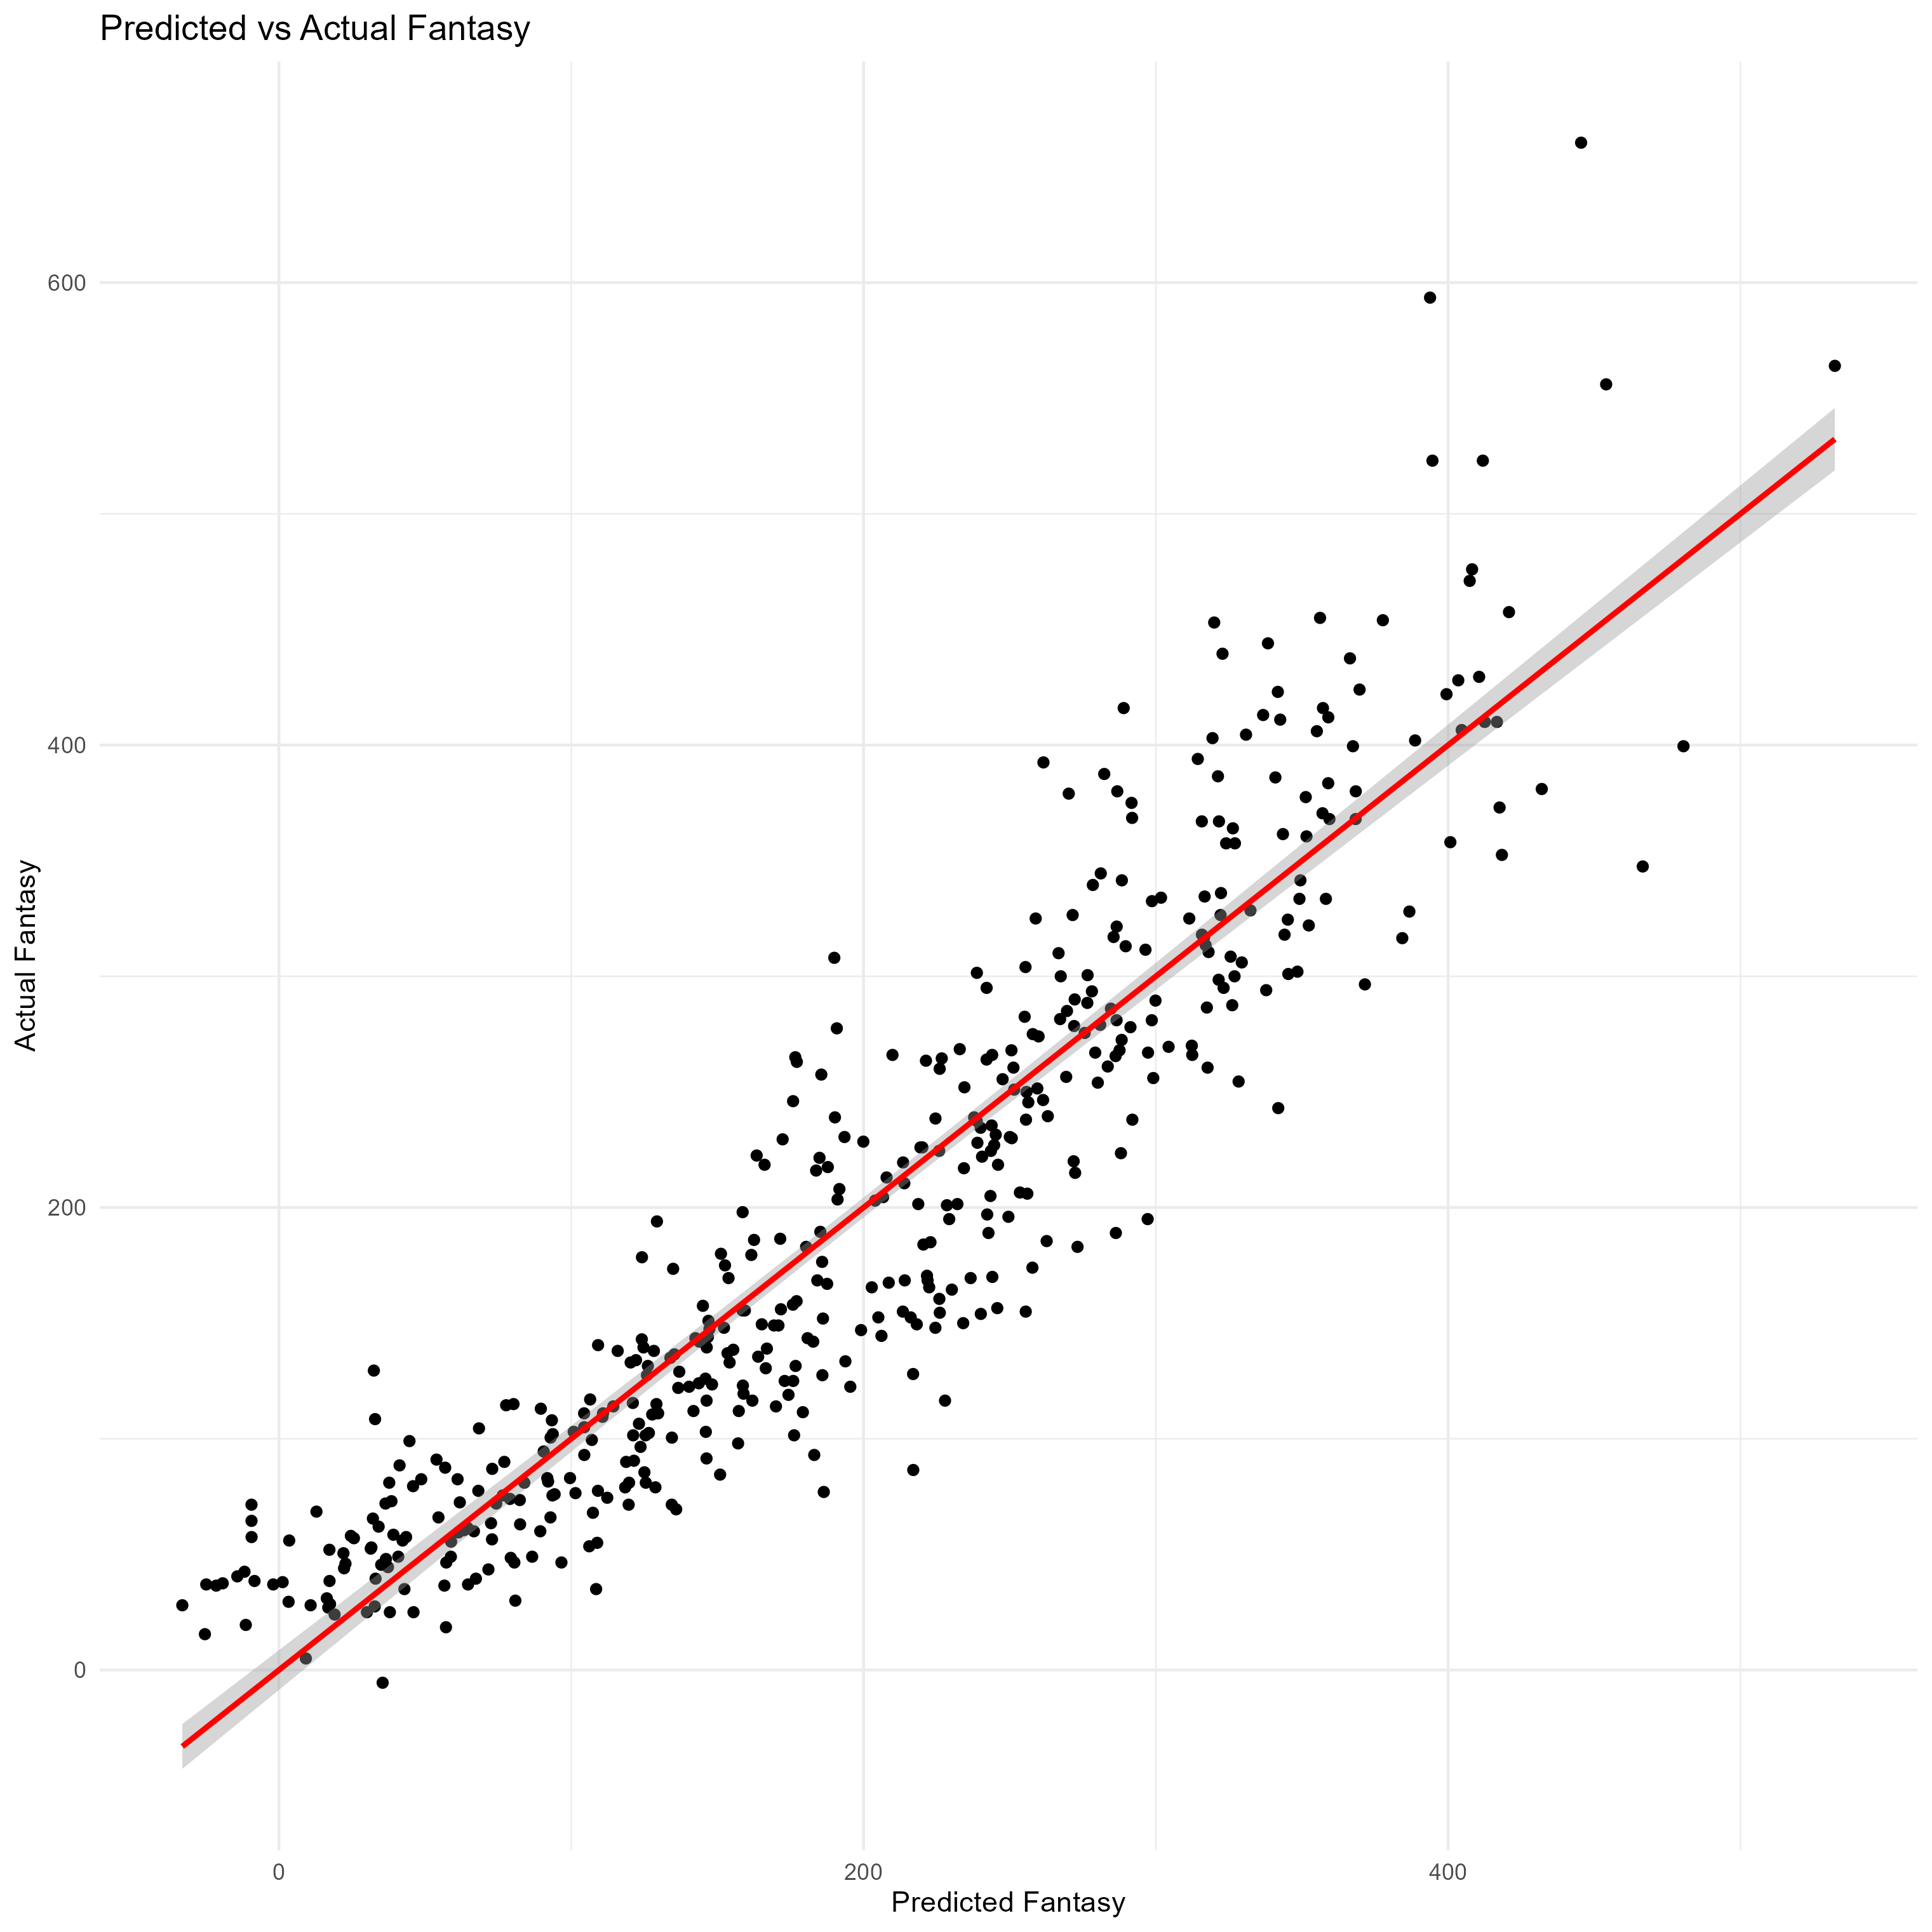
\includegraphics[width=15cm,height=10cm]{Predicted_vs_Actual_Fantasy_2023.png}
    \caption{Final Regression Model}
    \label{fig:figure B}
\end{figure}

\begin{figure}
    \centering
    \includegraphics[width=15cm,height=10cm]{forecasted_ops.png}
    \caption{OPS Regression}
    \label{fig:figure C}
\end{figure}

\begin{figure}
    \centering
    \includegraphics{moving_average.png}
    \caption{Moving Average OPS}
    \label{fig:figure D}
\end{figure}

\end{document}